\documentclass[11pt,a4paper]{article}
\usepackage[top=3cm,bottom=3cm,left=4cm,right=3cm]{geometry}
\usepackage[T1]{fontenc}
\usepackage{lmodern}
\usepackage{microtype}
\usepackage{amsmath}
\usepackage{amssymb}
\usepackage[htt]{hyphenat}
\usepackage{xurl}
\usepackage{graphicx}
\usepackage{caption}
\usepackage{float}
\usepackage{array}
\usepackage{tabularx}
\usepackage{enumitem}
\usepackage{xcolor}
\usepackage{tikz}
\usepackage{pgfplots}
\pgfplotsset{compat=1.16}
\usepackage{listings}
\usepackage{fancyhdr}
\usepackage[colorlinks=true,linkcolor=blue,urlcolor=blue]{hyperref}

% ---------------------------------------------------------------------------
% Istilah dalam Bahasa Indonesia (tanpa babel agar kompatibel di semua TeX)
% ---------------------------------------------------------------------------
\renewcommand{\contentsname}{Daftar Isi}
\renewcommand{\figurename}{Gambar}
\renewcommand{\tablename}{Tabel}
\renewcommand{\lstlistingname}{Kode}
\renewcommand{\appendixname}{Lampiran}
\renewcommand{\refname}{Daftar Pustaka}

% ---------------------------------------------------------------------------
% Header dan footer
% ---------------------------------------------------------------------------
\pagestyle{fancy}
\fancyhf{}
\fancyhead[L]{Modul 1 -- Identifikasi Sistem}
\fancyhead[R]{\nouppercase{\leftmark}}
\fancyfoot[L]{TF4015 Sistem Kontrol Diskrit}
\fancyfoot[R]{\thepage}
\renewcommand{\footrulewidth}{0.4pt}
\setlength{\headheight}{14pt}

% ---------------------------------------------------------------------------
% Gaya penulisan kode
% ---------------------------------------------------------------------------
\lstset{
	language=C++,
	basicstyle=\ttfamily\footnotesize,
	keywordstyle=\color{blue!70!black}\bfseries,
	commentstyle=\color{green!45!black},
	stringstyle=\color{red!65!black},
	numbers=left,
	numberstyle=\tiny\color{gray},
	frame=single,
	breaklines=true,
	tabsize=2,
	showstringspaces=false,
	columns=fullflexible,
	keepspaces=true,
	morekeywords={byte,uint32_t,String}
}

% ---------------------------------------------------------------------------
% Makro bantu
% ---------------------------------------------------------------------------
% Nama sketch utama program praktikum. Ubah di sini bila nama di repositori berbeda.
\newcommand{\sketch}{\texttt{SKD23.ino}}
% Nama file/program dalam teks
\newcommand{\prog}[1]{\texttt{#1}}
% Gambar dengan placeholder: bila file belum ada, ditampilkan kotak penanda
\newcommand{\gambar}[4]{%
	\begin{figure}[H]
		\centering
		\IfFileExists{#1}{%
			\includegraphics[width=#2]{#1}%
		}{%
			\fbox{\parbox[c][4cm][c]{0.7\textwidth}{\centering\small\textcolor{red}{Gambar belum tersedia:}\\\texttt{\detokenize{#1}}}}%
		}
		\caption{#3}
		\label{#4}
	\end{figure}}
% Kotak catatan / peringatan
\newcommand{\peringatan}[1]{%
	\begin{center}
		\fcolorbox{red!70!black}{red!5}{\parbox{0.92\textwidth}{\textbf{Peringatan.} #1}}
	\end{center}}
\newcommand{\catatan}[1]{%
	\begin{center}
		\fcolorbox{blue!60!black}{blue!4}{\parbox{0.92\textwidth}{\textbf{Catatan.} #1}}
	\end{center}}

\newcolumntype{C}{>{\centering\arraybackslash}X}
\setlength{\emergencystretch}{3em}
\setlist[itemize]{itemsep=2pt,topsep=4pt}
\setlist[enumerate]{itemsep=2pt,topsep=4pt}

\begin{document}

% ===========================================================================
% Halaman judul
% ===========================================================================
\begin{titlepage}
	\centering
	\vspace*{2cm}
	{\large TF4015 -- Sistem Kontrol Diskrit\par}
	\vspace{2.5cm}
	{\Large Praktikum\par}
	\vspace{0.4cm}
	{\huge\bfseries Modul 1\par}
	\vspace{0.4cm}
	{\LARGE Identifikasi Sistem\\Motor DC\par}
	\vfill
	% TODO: sesuaikan nama tim pengajar dan asisten
	{\large Tim Pengajar TF4015\par}
	\vspace{0.3cm}
	{\large Program Studi Teknik Fisika\\Fakultas Teknologi Industri\\Institut Teknologi Bandung\par}
	\vspace{0.8cm}
	{\large Semester I 2026/2027\par}
\end{titlepage}

\pagenumbering{roman}
\tableofcontents
\newpage
\pagenumbering{arabic}
\setcounter{page}{1}

% ===========================================================================
\section{Pendahuluan}
% ===========================================================================
\subsection{Latar Belakang}
Pengendalian kecepatan putar motor merupakan kasus inti pada berbagai aplikasi, seperti elevator, ban berjalan, dan pengaturan laju aliran fluida melalui pompa. Sebelum sebuah sistem dikendalikan secara kalang tertutup, perancang perlu mengetahui hubungan antara masukan dan keluaran sistem tersebut. Hubungan ini dapat diperoleh secara analitik dari hukum-hukum fisika, atau secara eksperimental dengan memberikan masukan tertentu lalu mengamati keluarannya. Pendekatan kedua disebut \textbf{identifikasi sistem}.

Pada Modul 1, praktikan belum melakukan pengontrolan. Seluruh percobaan dilakukan secara \textbf{kalang terbuka}. Praktikan terlebih dahulu mengamati karakteristik sensor, kemudian menentukan karakteristik statik motor, yaitu hubungan antara masukan dan kecepatan tunak. Dari karakteristik ini akan terlihat ketidaklinieran, seperti \textit{deadzone} dan saturasi, yang perlu diperbaiki dengan kompensasi sebelum sistem dikontrol.

Setelah dikompensasi, dinamika motor diidentifikasi dari respons step menggunakan model \textbf{orde satu dengan waktu tunda} (\textit{first order plus dead time}, FOPDT). Model ini kemudian digunakan untuk menentukan waktu cacah dan diturunkan menjadi model diskrit. Model kontinu dan model diskrit hasil Modul 1 menjadi dasar perancangan pengontrol kecepatan (Modul 2), kontrol posisi (Modul 3), dan \textit{pole placement} (Modul 4). Oleh karena itu, kualitas identifikasi pada modul ini akan sangat memengaruhi keberhasilan modul-modul berikutnya.

\subsection{Tujuan Praktikum}
Setelah menyelesaikan Modul 1, praktikan diharapkan mampu:
\begin{enumerate}
	\item Menganalisis karakteristik sensor posisi dan kecepatan, serta pengaruh metode akuisisi terhadap kualitas data dan waktu proses.
	\item Menyetel penguatan driver motor serta menentukan karakteristik statik dan spesifikasi kit praktikum.
	\item Merancang dan menerapkan fungsi kompensasi untuk mengurangi \textit{deadzone}.
	\item Mengidentifikasi parameter model FOPDT dari respons step sistem kecepatan motor DC.
	\item Menentukan waktu cacah, menurunkan model diskrit, dan memvalidasi model terhadap data percobaan.
\end{enumerate}

\subsection{Peralatan dan Perangkat Lunak}
\begin{table}[H]
	\centering
	\caption{Daftar peralatan praktikum Modul 1}
	\label{tab:peralatan}
	\begin{tabularx}{\textwidth}{|c|X|l|}
		\hline
		\textbf{No} & \textbf{Nama Peralatan}                                                    & \textbf{Keterangan}            \\
		\hline
		1           & Kit praktikum SKD (kit yang sama dengan Modul 0)                           & Disediakan asisten             \\
		2           & Obeng kecil untuk trimpot                                                  & Disediakan asisten             \\
		3           & Laptop dengan Arduino IDE dan \textit{library} Adafruit MCP4725            & Milik praktikan                \\
		4           & MATLAB (desktop atau MATLAB Online)                                        & Milik praktikan                \\
		5           & Perangkat lunak \textit{spreadsheet}                                       & Milik praktikan                \\
		6           & Program praktikum: \sketch, \prog{6\_main\_statik}, \prog{7\_main\_step}   & Unduh dari repositori          \\
		7           & Skrip MATLAB \prog{identifikasi\_fopdt.m}                                  & Unduh dari repositori          \\
		8           & Data dan laporan Modul 0 (terutama waktu proses $T_{proses}$)              & Hasil praktikum sebelumnya     \\
		\hline
	\end{tabularx}
\end{table}

\subsection{Persiapan Praktikum}
Sebelum praktikum, praktikan perlu:
\begin{enumerate}
	\item Menyelesaikan Modul 0 dan membawa hasil pengukuran waktu proses (Tabel perbandingan periode \texttt{loop()} pada Modul 0).
	\item Membaca Bagian~\ref{sec:teori} dan memahami program \prog{6\_main\_statik} serta \prog{7\_main\_step} (Lampiran~\ref{lamp:kode}).
	\item Membaca skrip \prog{identifikasi\_fopdt.m} dan mencobanya pada MATLAB, misalnya dengan data buatan sendiri.
	\item Menyiapkan templat \textit{spreadsheet} untuk tabel dan grafik pada modul ini.
	\item Membagi tugas dalam kelompok: pengoperasian kit, pencatatan data, dan pengolahan data dapat dilakukan secara paralel.
\end{enumerate}

% ===========================================================================
\section{Teori Dasar}
\label{sec:teori}
% ===========================================================================
\subsection{Karakteristik Statik dan Ketidaklinieran}
Karakteristik statik adalah hubungan antara masukan $u$ dan keluaran tunak $y_{ss}$ suatu sistem, $y_{ss} = f(u)$. Pada sistem ideal, hubungan ini linier. Pada kit praktikum, hubungan masukan motor (persen) dan kecepatan terukur (persen) memiliki beberapa ketidaklinieran, seperti diilustrasikan pada Gambar~\ref{fig:statik}:
\begin{itemize}
	\item \textbf{\textit{Deadzone}}: pada masukan kecil, motor belum berputar atau putarannya belum terbaca oleh sensor sehingga keluaran bernilai nol.
	\item \textbf{Saturasi}: pada masukan besar, kecepatan tidak bertambah lagi meskipun masukan dinaikkan.
	\item \textbf{Asimetri}: karakteristik untuk masukan positif dan negatif dapat berbeda.
\end{itemize}

\begin{figure}[H]
	\centering
	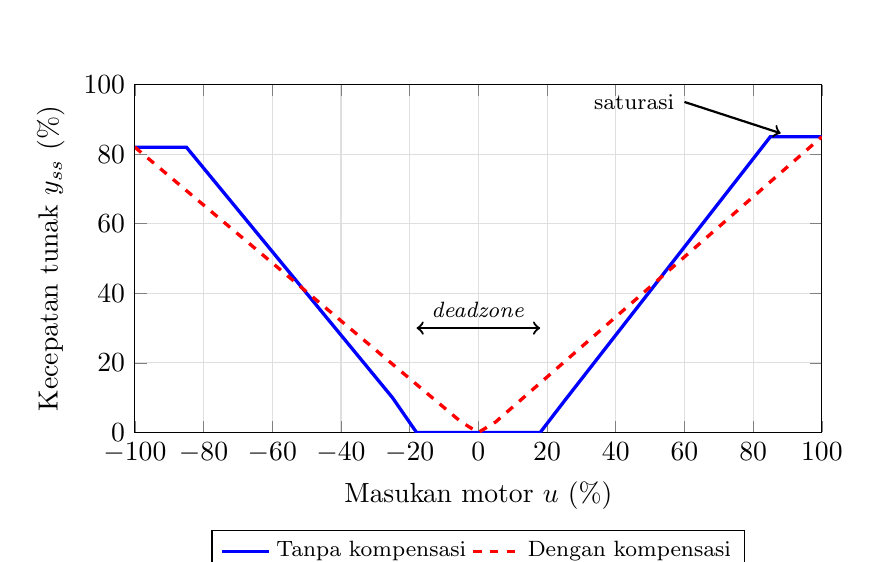
\begin{tikzpicture}
		\begin{axis}[
				width=0.85\textwidth, height=6cm,
				xmin=-100, xmax=100, ymin=0, ymax=100,
				xlabel={Masukan motor $u$ (\%)}, ylabel={Kecepatan tunak $y_{ss}$ (\%)},
				grid=major, grid style={gray!25},
				legend style={font=\footnotesize, at={(0.5,-0.28)}, anchor=north}, legend columns=2,
			]
			\addplot[very thick, blue] coordinates {(-100,82) (-85,82) (-25,10) (-18,0) (18,0) (25,9) (85,85) (100,85)};
			\addlegendentry{Tanpa kompensasi}
			\addplot[very thick, red, dashed] coordinates {(-100,82) (-5,3) (0,0) (5,3) (100,85)};
			\addlegendentry{Dengan kompensasi}
			\draw[<->, thick] (axis cs:-18,30) -- (axis cs:18,30) node[midway, above, font=\footnotesize] {\textit{deadzone}};
			\draw[->, thick] (axis cs:60,95) node[left, font=\footnotesize] {saturasi} -- (axis cs:88,86);
		\end{axis}
	\end{tikzpicture}
	\caption{Ilustrasi karakteristik statik motor dengan \textit{deadzone}, saturasi, dan efek kompensasi (bukan data sebenarnya). Bacaan tachometer selalu positif untuk kedua arah putar.}
	\label{fig:statik}
\end{figure}

Beberapa istilah spesifikasi yang digunakan pada modul ini:
\begin{itemize}
	\item \textbf{Masukan minimum putar motor}: masukan terkecil yang membuat motor mulai berputar. Putaran dapat dideteksi dari perubahan bacaan potensiometer walaupun tachometer masih membaca nol.
	\item \textbf{Masukan minimum terdeteksi}: masukan terkecil yang menghasilkan bacaan kecepatan tidak nol.
	\item \textbf{Masukan minimum putaran maksimal}: masukan terkecil yang sudah menghasilkan kecepatan maksimum (awal daerah saturasi).
\end{itemize}

Karakteristik statik dapat didekati dengan beberapa \textbf{daerah linier}, yaitu potongan garis lurus $y_{ss} \approx m_i u + c_i$ pada rentang masukan tertentu. Pembagian daerah minimal harus memperlihatkan daerah \textit{deadzone}, daerah naik, dan daerah saturasi. Kualitas pendekatan setiap daerah dapat dinilai dengan koefisien determinasi $R^2$. Pembagian yang terlalu banyak (lebih dari lima daerah) biasanya tidak lagi bermakna.

\subsection{Penguatan Driver Motor dan Saturasi}
Dari Modul 0, tegangan motor kurang lebih sebesar
\begin{equation}
	V_m \approx \min\!\left(A_v \cdot \frac{5\,|u|}{100} - V_{drop},\; V_{maks}\right),
	\qquad A_v = 1 + \frac{R_2}{R_1},
	\label{eq:vm}
\end{equation}
dengan $V_{drop}$ adalah rugi tegangan pada transistor dan L293D, dan $V_{maks}$ adalah tegangan maksimum yang dapat dicapai rangkaian (sedikit di bawah 24~V). Bila penguatan $A_v$ terlalu besar, tegangan maksimum sudah tercapai sebelum $u = 100\%$ sehingga rentang masukan di atasnya terbuang (saturasi dini). Bila $A_v$ terlalu kecil, kecepatan maksimum motor tidak pernah tercapai. Penguatan yang baik membuat kecepatan maksimum tercapai tepat ketika masukan mendekati 100\%. Penguatan diatur dengan trimpot $R_2$ pada rangkaian OpAmp.

\subsection{Kompensasi \textit{Deadzone}}
Kompensasi \textit{deadzone} bertujuan agar masukan kecil yang diberikan pengontrol langsung menghasilkan putaran. Caranya adalah memetakan masukan $u$ ke masukan terkompensasi $u_c$ yang melompati daerah \textit{deadzone}. Bentuk paling sederhana adalah pemetaan linier
\begin{equation}
	u_c =
	\begin{cases}
		DZ^{+} + u\,\dfrac{100 - DZ^{+}}{100}, & u > 0,  \\[2mm]
		0,                                      & u = 0,  \\[1mm]
		-DZ^{-} + u\,\dfrac{100 - DZ^{-}}{100}, & u < 0,
	\end{cases}
	\label{eq:kompensasi}
\end{equation}
dengan $DZ^{+}$ dan $DZ^{-}$ adalah besar \textit{deadzone} positif dan negatif dalam persen. Pemetaan ini menjaga $u_c = \pm 100$ ketika $u = \pm 100$. Persamaan~\eqref{eq:kompensasi} diimplementasikan pada tab \prog{4\_compensation.ino} melalui variabel \texttt{DeadZonePositif} dan \texttt{DeadZoneNegatif}. Pemilihan nilai $DZ$ (misalnya dari masukan minimum putar atau masukan minimum terdeteksi) merupakan keputusan rancangan yang perlu dijustifikasi.

\subsection{Model Orde Satu dengan Waktu Tunda}
Dinamika kecepatan motor DC beserta sensornya dapat didekati dengan model FOPDT
\begin{equation}
	G(s) = \frac{Y(s)}{U(s)} = \frac{K\,e^{-\theta s}}{\tau s + 1},
	\label{eq:fopdt}
\end{equation}
dengan $K$ adalah penguatan statik, $\tau$ adalah konstanta waktu, dan $\theta$ adalah waktu tunda. Untuk step masukan sebesar $\Delta U$ pada $t = 0$ dari keadaan tunak $Y_0$, respons model adalah
\begin{equation}
	y(t) =
	\begin{cases}
		Y_0,                                                         & t < \theta,   \\
		Y_0 + K\,\Delta U \left(1 - e^{-(t-\theta)/\tau}\right),     & t \ge \theta.
	\end{cases}
	\label{eq:respons_fopdt}
\end{equation}
Konstanta waktu terutama ditentukan oleh inersia mekanik motor, sedangkan waktu tunda dapat berasal dari gesekan, waktu komputasi, pencacahan, dan rangkaian pengkondisi sinyal sensor.

\subsection{Identifikasi Parameter dengan Metode Dua Titik}
Parameter model FOPDT diperoleh dari respons step (Gambar~\ref{fig:dua_titik}):
\begin{enumerate}
	\item \textbf{Penguatan}: $K = \Delta Y / \Delta U$, dengan $\Delta Y = Y_1 - Y_0$ adalah selisih keluaran tunak sesudah dan sebelum step, dan $\Delta U = U_1 - U_0$ adalah selisih masukan.
	\item \textbf{Konstanta waktu dan waktu tunda} (metode dua titik \cite{seborg}): tentukan waktu $t_{28}$ dan $t_{63}$ ketika respons mencapai $28{,}3\%$ dan $63{,}2\%$ dari $\Delta Y$, dihitung dari saat step diberikan. Dari Persamaan~\eqref{eq:respons_fopdt}, kedua titik ini memenuhi $t_{28} = \theta + \tau/3$ dan $t_{63} = \theta + \tau$, sehingga
	      \begin{equation}
		      \tau = 1{,}5\,(t_{63} - t_{28}), \qquad \theta = t_{63} - \tau.
		      \label{eq:dua_titik}
	      \end{equation}
\end{enumerate}

\begin{figure}[H]
	\centering
	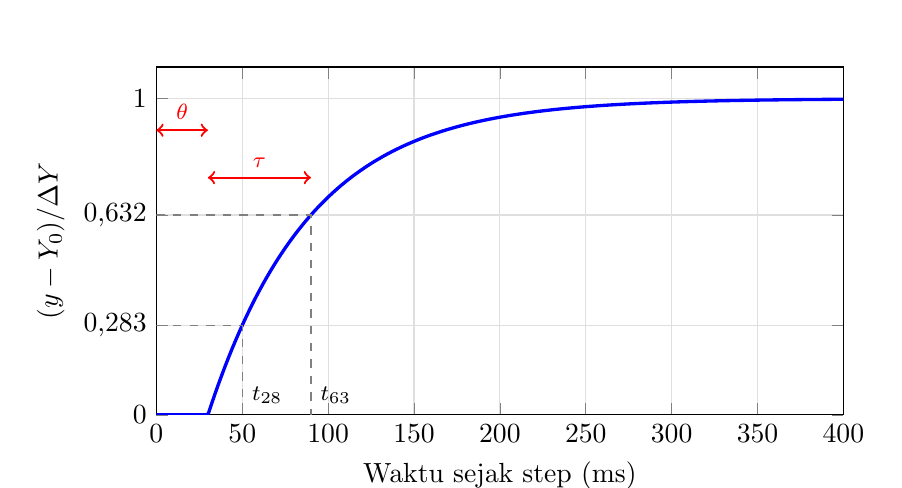
\begin{tikzpicture}
		\begin{axis}[
				width=0.85\textwidth, height=6cm,
				xmin=0, xmax=400, ymin=0, ymax=1.1,
				xlabel={Waktu sejak step (ms)}, ylabel={$(y - Y_0)/\Delta Y$},
				grid=major, grid style={gray!25},
				ytick={0,0.283,0.632,1}, yticklabels={0,{0,283},{0,632},1},
			]
			\addplot[very thick, blue, domain=0:400, samples=200] {x<30 ? 0 : 1-exp(-(x-30)/60)};
			\addplot[dashed, gray] coordinates {(0,0.283) (50,0.283) (50,0)};
			\addplot[dashed, gray] coordinates {(0,0.632) (90,0.632) (90,0)};
			\node[font=\footnotesize, anchor=north west] at (axis cs:50,0.12) {$t_{28}$};
			\node[font=\footnotesize, anchor=north west] at (axis cs:90,0.12) {$t_{63}$};
			\draw[<->, thick, red] (axis cs:0,0.9) -- (axis cs:30,0.9) node[midway, above, font=\footnotesize] {$\theta$};
			\draw[<->, thick, red] (axis cs:30,0.75) -- (axis cs:90,0.75) node[midway, above, font=\footnotesize] {$\tau$};
		\end{axis}
	\end{tikzpicture}
	\caption{Respons step ternormalisasi model FOPDT dan titik-titik yang digunakan pada metode dua titik ($\theta = 30$~ms, $\tau = 60$~ms)}
	\label{fig:dua_titik}
\end{figure}

Beberapa kesalahan yang sering terjadi dalam identifikasi:
\begin{itemize}
	\item Menggunakan nilai absolut masukan dan keluaran, bukan selisihnya, pada step yang tidak dimulai dari nol. Akibatnya nilai $K$ tidak sesuai.
	\item Menentukan saat step secara keliru sehingga waktu tunda bernilai negatif atau sangat kecil.
	\item Menahan masukan terlalu singkat sehingga keluaran belum mencapai keadaan tunak.
\end{itemize}

Karena sistem tidak sepenuhnya linier, parameter hasil identifikasi dapat berbeda untuk setiap besar masukan. Untuk keperluan perancangan, dipilih satu set parameter yang mewakili sistem, misalnya nilai rata-rata, median, atau nilai pada daerah kerja yang paling sering digunakan. Pilihan ini perlu dijustifikasi.

\subsection{Pemilihan Waktu Cacah}
Waktu cacah $T_s$ harus memenuhi dua batasan:
\begin{enumerate}
	\item \textbf{Batas bawah dari perangkat keras}: $T_s$ harus lebih besar daripada waktu proses satu siklus program, $T_s > T_{proses}$, dengan margin yang cukup (lihat hasil Modul 0).
	\item \textbf{Batas atas dari dinamika sistem}: $T_s$ harus cukup kecil agar dinamika sistem terwakili. Aturan praktis yang umum digunakan adalah memilih 4--10 sampel selama waktu naik $T_r$ \cite{astrom}. Untuk sistem orde satu, $T_r \approx 2{,}2\,\tau$, sehingga
	      \begin{equation}
		      \frac{T_r}{10} \le T_s \le \frac{T_r}{4}
		      \quad\Longrightarrow\quad
		      0{,}22\,\tau \lesssim T_s \lesssim 0{,}55\,\tau.
		      \label{eq:ts_rule}
	      \end{equation}
	      Bila pengontrol dirancang secara kontinu lalu didiskritkan (seperti pada Modul 2), waktu cacah yang lebih kecil, misalnya $T_s \approx \tau/10$, akan membuat perilaku pengontrol diskrit lebih mendekati rancangan kontinunya.
\end{enumerate}
Pada modul ini, praktikan menentukan \textbf{waktu cacah pertama} $T_{s1}$ dan \textbf{waktu cacah kedua} $T_{s2} = 3\,T_{s1}$. Kedua waktu cacah ini akan dibandingkan pada Modul 2.

\subsection{Model Diskrit}
Bila masukan ditahan konstan selama satu waktu cacah oleh DAC (\textit{zero-order hold}, ZOH) dan waktu tunda didekati sebagai kelipatan bulat waktu cacah, $\theta \approx d\,T_s$, model FOPDT~\eqref{eq:fopdt} memiliki padanan diskrit
\begin{equation}
	G(z) = \frac{b\,z^{-(d+1)}}{1 - a\,z^{-1}},
	\qquad a = e^{-T_s/\tau}, \quad b = K\,(1 - a), \quad d = \operatorname{round}\!\left(\frac{\theta}{T_s}\right),
	\label{eq:gz}
\end{equation}
atau dalam bentuk persamaan beda
\begin{equation}
	y[k+1] = a\,y[k] + b\,u[k-d].
	\label{eq:beda}
\end{equation}
Kutub sistem diskrit berada di $z = a$, yang selalu berada di dalam lingkaran satuan untuk $\tau > 0$. Penguatan tunak $G(1) = b/(1-a) = K$ tidak bergantung pada $T_s$. Model diskrit ini akan digunakan pada simulasi Modul 2 dan menjadi dasar perancangan \textit{pole placement} pada Modul 4.

% ===========================================================================
\section{Keselamatan Kerja}
% ===========================================================================
Seluruh ketentuan keselamatan kerja dan SOP pada Modul 0 tetap berlaku. Perhatikan pula hal-hal berikut yang khusus untuk Modul 1:
\begin{enumerate}
	\item Program \prog{6\_main\_statik} dan \prog{7\_main\_step} menjalankan motor secara otomatis selama beberapa menit. Jangan meninggalkan kit ketika program berjalan, dan cabut kabel listrik 220~V bila terjadi hal yang tidak diinginkan.
	\item Untuk arah negatif pada \prog{6\_main\_statik}, ubah \texttt{Sign} lalu unggah ulang program. Jangan membalik arah motor secara langsung.
	\item Gunakan hanya masukan positif pada urutan \texttt{Sequence[]} di \prog{7\_main\_step}.
	\item Putar trimpot perlahan menggunakan obeng kecil. Jangan menyentuh komponen lain pada PCB, terutama \textit{heat sink} transistor, ketika motor berputar.
	\item Variabel \texttt{DeadZonePositif} dan \texttt{DeadZoneNegatif} bertipe \texttt{byte}, sehingga harus diisi bilangan bulat positif 0--100. Nilai \textit{deadzone} negatif diisi besarnya saja.
\end{enumerate}

% ===========================================================================
\section{Prosedur Praktikum}
% ===========================================================================
Prosedur Modul 1 terdiri atas enam percobaan. Percobaan~1--5 menggunakan kit praktikum, sedangkan Percobaan~6 sebagian besar dikerjakan di MATLAB dan dapat dilakukan secara paralel. Simpan seluruh data mentah dari \textit{Serial Monitor} ke dalam file teks atau \textit{spreadsheet}.

\catatan{Data dari \textit{Serial Monitor} dapat disalin langsung (pilih seluruh teks, salin, lalu tempel ke file \texttt{.txt}). Alternatifnya, gunakan perangkat lunak terminal serial yang dapat menyimpan log ke file. Pastikan \textit{baudrate} 115200 dan pengaturan akhir baris \textbf{Newline}.}

\subsection{Percobaan 1: Karakteristik Sensor}
\textbf{Bagian A -- sensor posisi.} Kabel listrik 220~V tidak terhubung.
\begin{enumerate}
	\item Unggah program utama \prog{1\_main\_akuisisi\_data} dari Modul 0.
	\item Buka \textit{Serial Plotter}, lalu putar roda gigi potensiometer dengan tangan secara perlahan sebanyak satu putaran penuh, termasuk melewati titik ketika bacaan berpindah dari sekitar 100\% ke 0\% (atau sebaliknya). Simpan tangkapan layar.
	\item Biarkan potensiometer diam di sekitar 50\%. Rekam minimal 100 baris data, lalu hitung rata-rata dan simpangan baku kolom posisi satu sampel (Pos~2) dan posisi rata-rata (Pos~3).
\end{enumerate}

\textbf{Bagian B -- sensor kecepatan.}
\begin{enumerate}
	\item Unggah program utama \prog{5\_main\_motor} dari Modul 0, lalu hubungkan kabel listrik 220~V.
	\item Kirim masukan \texttt{75}. Setelah kecepatan tunak, rekam data selama sekitar 5 detik. Hitung rata-rata dan simpangan baku kolom kecepatan satu sampel (Kec~1) dan kecepatan rata-rata (Kec~2), serta rata-rata kolom \texttt{Delta}.
	\item Kirim \texttt{0}. Ubah jumlah sampel perataan pada fungsi \texttt{smooth\_velocity\_percentage()} di tab \prog{1\_sensor.ino} (argumen kedua \texttt{smooth\_pin}, bawaan 10) menjadi 1, 5, 20, dan 40. Untuk setiap nilai, ulangi langkah 2 dan lengkapi Tabel~\ref{tab:p1_sizeread}.
	\item Kembalikan jumlah sampel perataan ke nilai yang menurut kelompok paling sesuai, lalu gunakan nilai tersebut untuk percobaan selanjutnya.
\end{enumerate}

\catatan{Fungsi \texttt{smooth\_pin()} menjumlahkan hasil \texttt{analogRead()} ke variabel bertipe \texttt{unsigned int} (maksimum 65535). Jangan gunakan jumlah sampel lebih dari 64.}

\begin{table}[H]
	\centering
	\caption{Pengaruh jumlah sampel perataan terhadap bacaan kecepatan (masukan 75\%)}
	\label{tab:p1_sizeread}
	\begin{tabularx}{\textwidth}{|C|C|C|C|C|}
		\hline
		\textbf{Jumlah sampel} & \textbf{Rata-rata Kec (\%)} & \textbf{Simpangan baku Kec (\%)} & \textbf{Rata-rata \texttt{Delta} (ms)} & \textbf{Keterangan} \\
		\hline
		1                      &                             &                                  &                                        &                     \\
		5                      &                             &                                  &                                        &                     \\
		10                     &                             &                                  &                                        &                     \\
		20                     &                             &                                  &                                        &                     \\
		40                     &                             &                                  &                                        &                     \\
		\hline
	\end{tabularx}
\end{table}

\subsection{Percobaan 2: Penyetelan Penguatan Driver Motor}
\begin{enumerate}
	\item Dengan program \prog{5\_main\_motor}, kirim masukan \texttt{80}, \texttt{90}, \texttt{95}, dan \texttt{100} secara berurutan. Tunggu kecepatan tunak pada setiap masukan, lalu catat kecepatannya pada kolom ``sebelum'' Tabel~\ref{tab:p2_trimpot}.
	\item Bila kecepatan pada masukan 90\% atau 95\% sudah sama dengan kecepatan pada 100\%, penguatan terlalu besar. Dengan masukan \texttt{100}, putar trimpot sedikit demi sedikit sambil mengamati \textit{Serial Plotter} untuk menemukan arah putar yang menurunkan penguatan.
	\item Turunkan penguatan perlahan hingga kecepatan pada masukan 100\% \textbf{tepat mulai turun} dari nilai maksimumnya, lalu kembalikan sedikit hingga kecepatan maksimum tercapai lagi.
	\item Kirim kembali masukan \texttt{80}, \texttt{90}, \texttt{95}, dan \texttt{100}, lalu catat kecepatannya pada kolom ``sesudah''. Kecepatan pada 95\% seharusnya kini lebih kecil daripada kecepatan pada 100\%.
	\item Kirim \texttt{0}, lalu minta asisten memeriksa hasil penyetelan. \textbf{Jangan mengubah trimpot lagi} hingga akhir praktikum (termasuk Modul 2--4) karena model yang diidentifikasi bergantung pada penguatan ini.
\end{enumerate}

\begin{table}[H]
	\centering
	\caption{Kecepatan tunak sebelum dan sesudah penyetelan penguatan}
	\label{tab:p2_trimpot}
	\begin{tabular}{|c|c|c|}
		\hline
		\textbf{Masukan (\%)} & \textbf{Kecepatan sebelum (\%)} & \textbf{Kecepatan sesudah (\%)} \\
		\hline
		80                    &                                 &                                 \\
		90                    &                                 &                                 \\
		95                    &                                 &                                 \\
		100                   &                                 &                                 \\
		\hline
	\end{tabular}
\end{table}

\subsection{Percobaan 3: Karakteristik Statik Tanpa Kompensasi}
\begin{enumerate}
	\item Ganti tab \prog{9\_main.ino} dengan program \prog{6\_main\_statik} (Kode~\ref{lst:statik}). Atur \texttt{StepInput = 1}, \texttt{Sign = 1}, \texttt{UseCompensation = false}, dan \texttt{PrintAll = false}.
	\item Verifikasi program tanpa daya motor (kabel 220~V tidak terhubung) selama beberapa tingkat masukan, lalu unggah ulang program dan hubungkan kabel listrik. Program akan menaikkan masukan dari 0 hingga 100\% dengan setiap tingkat ditahan 2 detik (sekitar 3,5 menit).
	\item Setiap tingkat masukan menghasilkan satu baris: masukan, masukan motor, kecepatan tunak (rata-rata 1 detik terakhir), dan besar perubahan posisi selama tingkat tersebut. Salin seluruh hasil ke \textit{spreadsheet}.
	\item Cabut kabel listrik, ubah \texttt{Sign = -1}, unggah ulang, hubungkan kembali kabel listrik, lalu ulangi pengambilan data untuk arah negatif.
	\item Buat grafik hubungan masukan dan kecepatan tunak untuk kedua arah dalam satu grafik.
	\item Lengkapi Tabel~\ref{tab:p3_spesifikasi}. Gunakan kolom perubahan posisi untuk menentukan masukan minimum putar motor, dan kolom kecepatan tunak untuk menentukan masukan minimum terdeteksi. Gunakan simpangan baku dari Percobaan~1 sebagai acuan batas derau.
	\item Bagi karakteristik statik menjadi beberapa daerah linier dan lengkapi Tabel~\ref{tab:p3_linier}.
\end{enumerate}

\begin{table}[H]
	\centering
	\caption{Spesifikasi kit praktikum berkaitan dengan hubungan masukan dan kecepatan (Nomor kit: \underline{\hspace{1.5cm}})}
	\label{tab:p3_spesifikasi}
	\begin{tabularx}{\textwidth}{|c|X|c|c|}
		\hline
		\textbf{No} & \textbf{Spesifikasi}                         & \textbf{Nilai} & \textbf{Satuan} \\
		\hline
		1           & Masukan minimum putar motor (positif)        &                & \%              \\
		2           & Masukan minimum putar motor (negatif)        &                & \%              \\
		3           & Masukan minimum terdeteksi (positif)         &                & \%              \\
		4           & Masukan minimum terdeteksi (negatif)         &                & \%              \\
		5           & Masukan minimum putaran maksimal (positif)   &                & \%              \\
		6           & Masukan minimum putaran maksimal (negatif)   &                & \%              \\
		7           & Kecepatan putar maksimum (positif)           &                & \%              \\
		8           & Kecepatan putar maksimum (negatif)           &                & \%              \\
		\hline
	\end{tabularx}
\end{table}

\begin{table}[H]
	\centering
	\caption{Pembagian daerah linier karakteristik statik}
	\label{tab:p3_linier}
	\small
	\begin{tabularx}{\textwidth}{|c|C|C|c|c|X|}
		\hline
		\textbf{No} & \textbf{Rentang masukan (\%)} & \textbf{Rentang keluaran (\%)} & \textbf{$m$} & \textbf{$R^2$} & \textbf{Keterangan} \\
		\hline
		1           &                               &                                &                         &                &                     \\
		2           &                               &                                &                         &                &                     \\
		3           &                               &                                &                         &                &                     \\
		4           &                               &                                &                         &                &                     \\
		5           &                               &                                &                         &                &                     \\
		\hline
	\end{tabularx}
\end{table}

\subsection{Percobaan 4: Kompensasi \textit{Deadzone}}
\begin{enumerate}
	\item Berdasarkan Tabel~\ref{tab:p3_spesifikasi}, tentukan nilai $DZ^{+}$ dan $DZ^{-}$, lalu isi variabel \texttt{DeadZonePositif} dan \texttt{DeadZoneNegatif} pada tab \prog{4\_compensation.ino}. Bila diperlukan, kelompok boleh memodifikasi fungsi \texttt{compensation()} selama $u = 0$ tetap menghasilkan $u_c = 0$.
	\item Pada \prog{6\_main\_statik}, atur \texttt{UseCompensation = true}, \texttt{StepInput = 5}, dan \texttt{Sign = 1}. Verifikasi tanpa daya motor bahwa kolom \texttt{Motor} sesuai Persamaan~\eqref{eq:kompensasi}, lalu ambil data karakteristik statik.
	\item Ulangi untuk \texttt{Sign = -1}.
	\item Buat grafik karakteristik statik dengan dan tanpa kompensasi dalam satu gambar, lalu lengkapi kembali tabel daerah linier (gunakan format Tabel~\ref{tab:p3_linier}) untuk sistem terkompensasi.
	\item Bila \textit{deadzone} belum berkurang setidaknya setengahnya, perbaiki nilai $DZ$ atau fungsi kompensasi, lalu ulangi langkah 2--3.
\end{enumerate}

\subsection{Percobaan 5: Respons Step}
\begin{enumerate}
	\item Ganti tab \prog{9\_main.ino} dengan program \prog{7\_main\_step} (Kode~\ref{lst:step}). Pastikan \texttt{UseCompensation = true} dan fungsi kompensasi dari Percobaan~4 sudah digunakan.
	\item Atur \texttt{TimeSampling} sekecil mungkin tetapi tetap lebih besar daripada waktu proses (misalnya 10~ms). Periksa kolom \texttt{Delta} untuk memastikan waktu cacah konsisten.
	\item \textbf{Data A -- step dari nol}: gunakan urutan \texttt{\{0, 20, 0, 40, 0, 60, 0, 80, 0, 100, 0\}}. Verifikasi tanpa daya motor, lalu jalankan dan simpan seluruh data ke file \prog{data\_A.txt}.
	\item Periksa apakah kecepatan sudah tunak sebelum masukan berikutnya. Bila belum, perbesar \texttt{HoldTime} dan ulangi.
	\item \textbf{Data B -- step berkelanjutan}: gunakan urutan \texttt{\{0, 20, 40, 60, 80, 100, 0\}}, lalu simpan ke file \prog{data\_B.txt}.
\end{enumerate}

\subsection{Percobaan 6: Identifikasi Model, Waktu Cacah, dan Model Diskrit}
\begin{enumerate}
	\item Buka skrip \prog{identifikasi\_fopdt.m} (Kode~\ref{lst:matlab}). Atur \texttt{NamaFile = 'data\_A.txt'}, lalu jalankan. Skrip akan menampilkan parameter $K$, $\tau$, dan $\theta$ untuk setiap step naik. Lengkapi Tabel~\ref{tab:p6_identifikasi}.
	\item Ulangi untuk \prog{data\_B.txt}.
	\item Periksa hasil skrip dengan menghitung secara manual parameter salah satu step menggunakan \textit{spreadsheet} dan Persamaan~\eqref{eq:dua_titik}.
	\item Tentukan satu set parameter $K$, $\tau$, dan $\theta$ yang mewakili sistem, lalu tentukan $T_{s1}$ berdasarkan Persamaan~\eqref{eq:ts_rule} dan waktu proses dari Modul 0. Tetapkan $T_{s2} = 3\,T_{s1}$. Lengkapi Tabel~\ref{tab:p6_model}.
	\item Isi parameter tersebut pada bagian parameter manual skrip, ubah variabel \texttt{GunakanParameterManual} menjadi \texttt{true}, dan isi nilai \texttt{Ts1}. Catat koefisien $a$, $b$, dan $d$ model diskrit yang ditampilkan.
	\item \textbf{Validasi}: atur \texttt{TimeSampling} pada \prog{7\_main\_step} menjadi $T_{s1}$, ambil kembali data dengan urutan Data A, lalu jalankan skrip pada data baru tersebut. Catat nilai RMSE dan simpan grafik perbandingan. Ulangi untuk $T_{s2}$. Lengkapi Tabel~\ref{tab:p6_validasi}.
\end{enumerate}

\begin{table}[H]
	\centering
	\caption{Hasil identifikasi parameter setiap step}
	\label{tab:p6_identifikasi}
	\small
	\begin{tabularx}{\textwidth}{|c|c|C|C|C|C|X|}
		\hline
		\textbf{Data} & \textbf{Step} & \textbf{$\Delta Y$ (\%)} & \textbf{$K$} & \textbf{$\tau$ (ms)} & \textbf{$\theta$ (ms)} & \textbf{Ket.} \\
		\hline
		A             & $0 \rightarrow 20$                    &                          &              &                      &                        &                     \\
		A             & $0 \rightarrow 40$                    &                          &              &                      &                        &                     \\
		A             & $0 \rightarrow 60$                    &                          &              &                      &                        &                     \\
		A             & $0 \rightarrow 80$                    &                          &              &                      &                        &                     \\
		A             & $0 \rightarrow 100$                   &                          &              &                      &                        &                     \\
		\hline
		B             & $0 \rightarrow 20$                    &                          &              &                      &                        &                     \\
		B             & $20 \rightarrow 40$                   &                          &              &                      &                        &                     \\
		B             & $40 \rightarrow 60$                   &                          &              &                      &                        &                     \\
		B             & $60 \rightarrow 80$                   &                          &              &                      &                        &                     \\
		B             & $80 \rightarrow 100$                  &                          &              &                      &                        &                     \\
		\hline
	\end{tabularx}
\end{table}

\begin{table}[H]
	\centering
	\caption{Model final sistem kecepatan kit praktikum}
	\label{tab:p6_model}
	\begin{tabularx}{\textwidth}{|c|l|c|c|X|}
		\hline
		\textbf{No} & \textbf{Parameter}                   & \textbf{Nilai} & \textbf{Satuan} & \textbf{Model} \\
		\hline
		1           & Penguatan $K$                        &                & --              &                \\
		2           & Konstanta waktu $\tau$               &                & ms              &                \\
		3           & Waktu tunda $\theta$                 &                & ms              &                \\
		4           & Kecepatan maksimum                   &                & \%              &                \\
		5           & Waktu cacah pertama $T_{s1}$         &                & ms              &                \\
		6           & $a$, $b$, $d$ untuk $T_{s1}$         &                & --              &                \\
		7           & Waktu cacah kedua $T_{s2}$           &                & ms              &                \\
		8           & $a$, $b$, $d$ untuk $T_{s2}$         &                & --              &                \\
		\hline
	\end{tabularx}
\end{table}

\begin{table}[H]
	\centering
	\caption{Validasi model diskrit terhadap data percobaan}
	\label{tab:p6_validasi}
	\begin{tabular}{|c|c|c|}
		\hline
		\textbf{Waktu cacah} & \textbf{Nilai (ms)} & \textbf{RMSE (\%)} \\
		\hline
		$T_{s1}$             &                     &                    \\
		$T_{s2}$             &                     &                    \\
		\hline
	\end{tabular}
\end{table}

% ===========================================================================
\section{Laporan dan Analisis}
% ===========================================================================
\subsection{Ketentuan Laporan}
% TODO: sesuaikan platform dan tenggat pengumpulan
Laporan dikumpulkan per kelompok melalui Edunex paling lambat dua minggu setelah praktikum. Nilai tambahan diberikan bila laporan dikumpulkan dalam satu minggu. Laporan berupa file \texttt{.pdf} yang dilampiri \textit{spreadsheet} pengolahan data, data mentah (\texttt{.txt}), program Arduino yang dimodifikasi, dan skrip MATLAB, digabung dalam satu file \texttt{.zip}. Laporan minimal memiliki susunan berikut: latar belakang, tujuan, alat, prosedur, analisis, kesimpulan, kontribusi, dan referensi.

Latar belakang, tujuan, alat, dan prosedur tidak boleh sama persis dengan modul ini; tuliskan kembali sesuai pemahaman kelompok dan pelaksanaan yang sebenarnya. Analisis disusun dengan alur yang runtut dengan menjawab pertanyaan pada Bagian~\ref{sec:analisis}; urutan jawaban tidak harus sama dengan urutan pertanyaan. Perhatikan penggunaan angka penting pada setiap hasil perhitungan. Bagian kontribusi berisi Tabel~\ref{tab:kontribusi}.

\begin{table}[H]
	\centering
	\caption{Kontribusi anggota kelompok}
	\label{tab:kontribusi}
	\begin{tabularx}{\textwidth}{|c|c|l|X|}
		\hline
		\textbf{No} & \textbf{NIM} & \textbf{Nama Lengkap} & \textbf{Kontribusi} \\
		\hline
		1           &              &                       &                     \\
		2           &              &                       &                     \\
		3           &              &                       &                     \\
		4           &              &                       &                     \\
		5           &              &                       &                     \\
		\hline
	\end{tabularx}
\end{table}

\subsection{Analisis}
\label{sec:analisis}

\paragraph{Karakteristik sensor.}
\begin{enumerate}
	\item Tunjukkan grafik bacaan potensiometer ketika diputar satu putaran penuh. Jelaskan mengapa bacaan berpindah langsung dari sekitar 100\% ke 0\% (atau sebaliknya). Apa konsekuensinya bagi kontrol posisi pada Modul 3?
	\item Jelaskan kelebihan dan kekurangan akuisisi satu sampel (\texttt{sample}) dan perataan beberapa sampel (\texttt{smooth}) berdasarkan Tabel~\ref{tab:p1_sizeread}. Berapa jumlah sampel perataan yang kelompok pilih, dan apa pertimbangannya?
	\item Mengapa jumlah sampel perataan tidak boleh lebih dari 64?
	\item Apa saja yang memengaruhi waktu proses satu siklus program? Bagaimana cara mengoptimalkannya?
\end{enumerate}

\paragraph{Penyetelan penguatan dan karakteristik statik.}
\begin{enumerate}[resume]
	\item Jelaskan bagaimana trimpot pada rangkaian OpAmp memengaruhi kecepatan maksimum motor berdasarkan Persamaan~\eqref{eq:vm} dan Tabel~\ref{tab:p2_trimpot}. Mengapa penyetelan ini penting sebelum identifikasi?
	\item Bacaan kecepatan selalu positif, baik untuk masukan positif maupun negatif. Mengapa demikian? Bagaimana tanda masukan memengaruhi arah putar motor?
	\item Mengapa motor tidak berputar ketika masukan kecil? Mengapa bacaan kecepatan dapat bernilai nol walaupun motor sudah berputar pelan? Kaitkan dengan rangkaian pengkondisi sinyal tachometer pada Modul 0.
	\item Tunjukkan grafik karakteristik statik tanpa kompensasi dan Tabel~\ref{tab:p3_spesifikasi}. Apakah karakteristik arah positif dan negatif simetris?
	\item Jelaskan pembagian daerah linier yang dipilih beserta pertimbangannya (Tabel~\ref{tab:p3_linier}).
\end{enumerate}

\paragraph{Kompensasi \textit{deadzone}.}
\begin{enumerate}[resume]
	\item Gambarkan diagram blok kit praktikum untuk sistem kalang terbuka dan kalang terbuka terkompensasi. Jelaskan perbedaannya.
	\item Jelaskan fungsi kompensasi yang digunakan dan tuliskan dalam persamaan matematika. Mengapa kelompok memilih nilai $DZ^{+}$ dan $DZ^{-}$ tersebut? Apa akibatnya bila $DZ$ dipilih terlalu kecil atau terlalu besar?
	\item Tunjukkan grafik karakteristik statik dengan dan tanpa kompensasi dalam satu gambar. Apakah kompensasi berhasil mengurangi \textit{deadzone}? Bandingkan pembagian daerah liniernya.
\end{enumerate}

\paragraph{Identifikasi model.}
\begin{enumerate}[resume]
	\item Tunjukkan respons step Data A dan Data B beserta Tabel~\ref{tab:p6_identifikasi}. Buat grafik parameter $K$, $\tau$, dan $\theta$ terhadap besar masukan. Bagaimana parameter berubah terhadap titik kerja, dan apa artinya bagi asumsi linier?
	\item Bandingkan hasil identifikasi step dari nol dan step berkelanjutan. Metode mana yang lebih sesuai untuk kit ini? Jelaskan.
	\item Bandingkan hasil skrip dengan perhitungan manual. Apakah terdapat waktu tunda yang bernilai negatif atau sangat kecil? Jika ya, apa penyebabnya?
	\item Pilih satu set parameter yang mewakili sistem dan jelaskan dasar pemilihannya.
	\item Identifikasi secara manual konstanta waktu pada salah satu step \textbf{turun} (misalnya $100 \rightarrow 0$ pada Data A). Bandingkan dengan konstanta waktu step naik dan dengan konstanta waktu filter tachometer pada Modul 0 ($\tau_f = 0{,}1$~s). Apa yang dapat disimpulkan?
\end{enumerate}

\paragraph{Waktu cacah dan model diskrit.}
\begin{enumerate}[resume]
	\item Jelaskan pertimbangan pemilihan $T_{s1}$. Apakah $T_{s1}$ dan $T_{s2}$ memenuhi Persamaan~\eqref{eq:ts_rule}?
	\item Tuliskan model diskrit $G(z)$ untuk $T_{s1}$ dan $T_{s2}$. Di mana letak kutubnya? Bagaimana letak kutub berubah bila waktu cacah diperbesar?
	\item Tunjukkan grafik validasi dan Tabel~\ref{tab:p6_validasi}. Apakah model diskrit cukup mewakili kit praktikum? Pada kondisi apa model paling berbeda dengan data, dan mengapa?
\end{enumerate}

% ===========================================================================
\section{Tugas Tambahan}
% ===========================================================================
Tugas tambahan bersifat opsional dan dapat ditambahkan pada laporan untuk nilai tambah. Tugas ini juga merupakan persiapan Modul 2.
\begin{enumerate}
	\item Hitung parameter pengontrol P, PI, dan PID menggunakan metode Ziegler--Nichols dan Cohen--Coon berdasarkan model final untuk kedua waktu cacah.
	\item Simulasikan respons kalang terbuka dan kalang tertutup menggunakan program simulasi MATLAB yang disediakan. Pengontrol mana yang paling sesuai? Berikan justifikasi.
	\item Identifikasi model orde dua dengan waktu tunda dari data yang sama, lalu bandingkan RMSE-nya dengan model FOPDT. Apakah peningkatan akurasinya sepadan dengan bertambahnya kompleksitas model?
	\item Siapkan fungsi pada tab \prog{5\_control.ino} untuk menghitung aksi kontrol PID diskrit beserta program utama yang mengontrol kecepatan motor sesuai masukan serial.
\end{enumerate}

% ===========================================================================
\begin{thebibliography}{9}
	\bibitem{astrom} K.~J. Åström dan B.~Wittenmark, \textit{Computer-Controlled Systems: Theory and Design}, edisi ke-3. Englewood Cliffs, NJ: Prentice Hall, 1997.
	\bibitem{seborg} D.~E. Seborg, T.~F. Edgar, D.~A. Mellichamp, dan F.~J. Doyle III, \textit{Process Dynamics and Control}, edisi ke-4. Hoboken, NJ: Wiley, 2016.
\end{thebibliography}

% ===========================================================================
\clearpage
\appendix
\section{Kode Program Pendukung}
\label{lamp:kode}
% ===========================================================================
Program utama berikut menggantikan isi tab \prog{9\_main.ino}. Tab lain (\prog{1\_sensor.ino} hingga \prog{4\_compensation.ino}) tetap sama seperti pada Modul 0.

\begin{lstlisting}[caption={Program utama \texttt{6\_main\_statik}},label={lst:statik}]
// ===========================================================================
// Program utama Modul 1: karakteristik statik (masukan bertingkat)
// Ganti isi tab 9_main.ino dengan program ini.
//
// Masukan motor dinaikkan bertahap dari 0 hingga 100% (atau 0 hingga -100%
// bila Sign = -1). Setiap tingkat ditahan selama HoldTime. Kecepatan tunak
// dihitung sebagai rata-rata bacaan kecepatan pada AverageTime terakhir.
// Untuk arah negatif, ubah Sign menjadi -1 lalu unggah ulang program
// (jangan membalik arah motor secara langsung).
// ===========================================================================

unsigned long Time, StartTime, LastTime, LevelStart;
unsigned int TimeSampling = 20, DeltaTime;   // waktu cacah (ms)
unsigned int HoldTime = 2000;                // lama tiap tingkat masukan (ms)
unsigned int AverageTime = 1000;             // rentang akhir tiap tingkat untuk rata-rata (ms)
int StepInput = 1;                           // kenaikan masukan tiap tingkat (%)
int Sign = 1;                                // 1: arah positif, -1: arah negatif
bool UseCompensation = false;                // true: masukan dikompensasi (Percobaan 4)
bool PrintAll = false;                       // true: cetak semua sampel, false: ringkasan tiap tingkat

int Level = 0;
float InputLevel = 0.0, MotorInput = 0.0, Motor = 0.0;
float Speed = 0.0, Position = 0.0, PositionStart = 0.0;
float SumSpeed = 0.0;
unsigned int CountSpeed = 0;
bool Finished = false;

void setup() {
  general_setup();
  sensor_setup();
  actuator_setup();
  print_header();
  StartTime = millis();
  LastTime = StartTime;
  LevelStart = StartTime;
  PositionStart = smooth_position_percentage();
}

void loop() {
  Time = millis();
  if (Time - LastTime >= TimeSampling) {
    DeltaTime = Time - LastTime;
    LastTime = Time;

    if (Finished) {
      run_motor(0.0);
      return;
    }

    InputLevel = (float) (Sign * Level * StepInput);
    if (UseCompensation) MotorInput = compensation(InputLevel);
    else MotorInput = InputLevel;
    Motor = run_motor(MotorInput);

    Speed = smooth_velocity_percentage();
    Position = smooth_position_percentage();

    if (Time - LevelStart >= (unsigned long) (HoldTime - AverageTime)) {
      SumSpeed += Speed;
      CountSpeed++;
    }

    if (PrintAll) print_sample();

    if (Time - LevelStart >= HoldTime) {
      if (!PrintAll) print_summary();
      SumSpeed = 0.0;
      CountSpeed = 0;
      LevelStart = Time;
      PositionStart = Position;
      Level++;
      if (Level * StepInput > 100) {
        Finished = true;
        Serial.println("# selesai");
      }
    }
  }
}

void print_header() {
  if (PrintAll) Serial.println("Time\tDelta\tInput\tMotor\tKec\tPos");
  else Serial.println("Input\tMotor\tKecTunak\tPerubahanPos");
}

void print_sample() {
  Serial.print(Time - StartTime);
  Serial.print("\t");
  Serial.print(DeltaTime);
  Serial.print("\t");
  Serial.print(InputLevel);
  Serial.print("\t");
  Serial.print(Motor);
  Serial.print("\t");
  Serial.print(Speed);
  Serial.print("\t");
  Serial.println(Position);
}

void print_summary() {
  float PositionChange = Position - PositionStart;
  if (PositionChange < 0) PositionChange = -PositionChange;
  Serial.print(InputLevel);
  Serial.print("\t");
  Serial.print(Motor);
  Serial.print("\t");
  if (CountSpeed > 0) Serial.print(SumSpeed / CountSpeed);
  else Serial.print(Speed);
  Serial.print("\t");
  Serial.println(PositionChange);
}
\end{lstlisting}

\begin{lstlisting}[caption={Program utama \texttt{7\_main\_step}},label={lst:step}]
// ===========================================================================
// Program utama Modul 1: respons step untuk identifikasi dinamika
// Ganti isi tab 9_main.ino dengan program ini.
//
// Masukan motor mengikuti urutan Sequence[]; setiap nilai ditahan selama
// HoldTime. Data waktu, masukan, dan kecepatan dicetak setiap waktu cacah
// sehingga dapat disalin ke spreadsheet dan diolah dengan MATLAB.
//
// Contoh urutan:
//   step dari nol      : {0, 20, 0, 40, 0, 60, 0, 80, 0, 100, 0}
//   step berkelanjutan : {0, 20, 40, 60, 80, 100, 0}
// Gunakan masukan positif saja agar arah motor tidak berbalik.
// ===========================================================================

unsigned long Time, StartTime, LastTime, StepStart;
unsigned int TimeSampling = 10, DeltaTime;   // waktu cacah (ms)
unsigned int HoldTime = 2000;                // lama tiap nilai masukan (ms)
bool UseCompensation = true;                 // gunakan kompensasi deadzone dari Percobaan 4

int Sequence[] = {0, 20, 0, 40, 0, 60, 0, 80, 0, 100, 0};
const byte SequenceLength = sizeof(Sequence) / sizeof(Sequence[0]);

byte Index = 0;
float InputStep = 0.0, MotorInput = 0.0, Motor = 0.0, Speed = 0.0;
bool Finished = false;

void setup() {
  general_setup();
  sensor_setup();
  actuator_setup();
  Serial.println("Time\tDelta\tInput\tMotor\tKec");
  StartTime = millis();
  LastTime = StartTime;
  StepStart = StartTime;
}

void loop() {
  Time = millis();
  if (Time - LastTime >= TimeSampling) {
    DeltaTime = Time - LastTime;
    LastTime = Time;

    if (Finished) {
      run_motor(0.0);
      return;
    }

    InputStep = (float) Sequence[Index];
    if (UseCompensation) MotorInput = compensation(InputStep);
    else MotorInput = InputStep;
    Motor = run_motor(MotorInput);
    Speed = smooth_velocity_percentage();

    Serial.print(Time - StartTime);
    Serial.print("\t");
    Serial.print(DeltaTime);
    Serial.print("\t");
    Serial.print(InputStep);
    Serial.print("\t");
    Serial.print(Motor);
    Serial.print("\t");
    Serial.println(Speed);

    if (Time - StepStart >= HoldTime) {
      StepStart = Time;
      Index++;
      if (Index >= SequenceLength) {
        Finished = true;
        Serial.println("# selesai");
      }
    }
  }
}
\end{lstlisting}

\begin{lstlisting}[language=Matlab, morekeywords={readmatrix,movmean,array2table,warning,stairs}, caption={Skrip MATLAB \texttt{identifikasi\_fopdt.m}},label={lst:matlab}]
%% identifikasi_fopdt.m
% Identifikasi model orde satu dengan waktu tunda (FOPDT) dari data respons
% step kit praktikum Sistem Kontrol Diskrit (Modul 1).
%
% Data berasal dari program utama 7_main_step yang disalin dari Serial
% Monitor ke file teks (.txt) atau .csv dengan kolom:
%   Time (ms) | Delta (ms) | Input (%) | Motor (%) | Kec (%)
%
% Skrip ini:
%   1. mencari setiap step masukan naik (Delta U > 0),
%   2. menghitung K, tau, dan theta setiap step dengan metode dua titik
%      (28,3% dan 63,2%),
%   3. menghitung model diskrit (ZOH) untuk dua waktu cacah,
%   4. membandingkan respons model diskrit dengan data.

clc; clear; close all;

%% 1. Pengaturan
NamaFile      = 'data_step.txt';  % nama file data
KolomWaktu    = 1;                % kolom waktu (ms)
KolomMasukan  = 3;                % kolom masukan (%)
KolomKeluaran = 5;                % kolom kecepatan (%)
FraksiTunak   = 0.3;              % porsi akhir tiap segmen untuk nilai tunak
LebarFilter   = 3;                % lebar rata-rata bergerak untuk mencari titik lintas

Ts1 = 10;                         % waktu cacah pertama (ms), ubah sesuai pilihan kelompok
Ts2 = 3*Ts1;                      % waktu cacah kedua (ms)

% Parameter manual: isi dengan model final kelompok untuk memvalidasi model
% pada data baru (Percobaan 6). Bila false, digunakan median hasil step.
GunakanParameterManual = false;
K_manual     = 0.9;               % (-)
Tau_manual   = 60;                % (ms)
Theta_manual = 30;                % (ms)

%% 2. Membaca data
Data = readmatrix(NamaFile);
Kolom = [KolomWaktu KolomMasukan KolomKeluaran];
Data = Data(all(~isnan(Data(:, Kolom)), 2), :);   % buang baris teks / kosong
t = Data(:, KolomWaktu);
u = Data(:, KolomMasukan);
y = Data(:, KolomKeluaran);
t = t - t(1);
N = numel(t);

%% 3. Identifikasi parameter setiap step naik
IndeksStep = find(diff(u) ~= 0) + 1;     % sampel pertama setelah masukan berubah
Batas = [1; IndeksStep; N + 1];          % segmen ke-j: Batas(j) .. Batas(j+1)-1

Hasil = [];
for i = 1:numel(IndeksStep)
    SegSebelum = Batas(i):Batas(i+1)-1;
    SegSesudah = Batas(i+1):Batas(i+2)-1;
    U0 = u(SegSebelum(1));
    U1 = u(SegSesudah(1));
    dU = U1 - U0;
    if dU <= 0
        continue;                        % hanya step naik yang diidentifikasi
    end

    Y0 = mean(y(SegSebelum(end - porsi(numel(SegSebelum), FraksiTunak) + 1:end)));
    Y1 = mean(y(SegSesudah(end - porsi(numel(SegSesudah), FraksiTunak) + 1:end)));
    dY = Y1 - Y0;
    K  = dY / dU;

    tt = t(SegSesudah) - t(SegSesudah(1));
    r  = (movmean(y(SegSesudah), LebarFilter) - Y0) / dY;   % respons ternormalisasi
    t28 = waktu_lintas(tt, r, 0.283);
    t63 = waktu_lintas(tt, r, 0.632);
    Tau   = 1.5 * (t63 - t28);
    Theta = t63 - Tau;
    if Theta < 0
        warning('Step %g -> %g: waktu tunda negatif (%.1f ms), periksa data.', U0, U1, Theta);
    end

    Hasil(end+1, :) = [U0 U1 dU Y0 Y1 dY K Tau Theta]; %#ok<SAGROW>
end

if isempty(Hasil)
    error('Tidak ditemukan step masukan naik pada data.');
end

TabelHasil = array2table(Hasil, 'VariableNames', ...
    {'U0','U1','dU','Y0','Y1','dY','K','Tau_ms','Theta_ms'});
disp('Hasil identifikasi setiap step:');
disp(TabelHasil);

%% 4. Nilai yang mewakili sistem
% Secara bawaan digunakan median. Ganti dengan nilai pilihan kelompok bila
% ada alasan yang lebih kuat (misalnya hanya memakai daerah linier).
if GunakanParameterManual
    K     = K_manual;
    Tau   = Tau_manual;
    Theta = Theta_manual;
else
    K     = median(Hasil(:, 7));
    Tau   = median(Hasil(:, 8));
    Theta = max(median(Hasil(:, 9)), 0);
end
fprintf('\nModel kontinu: G(s) = %.3f e^(-%.1f s) / (%.1f s + 1)   [s dalam ms]\n', ...
    K, Theta, Tau);

%% 5. Model diskrit (ZOH) untuk dua waktu cacah
fprintf('\nModel diskrit y[k+1] = a y[k] + b u[k-d]:\n');
for Ts = [Ts1 Ts2]
    a = exp(-Ts / Tau);
    b = K * (1 - a);
    d = round(Theta / Ts);
    fprintf('  Ts = %3g ms : a = %.4f, b = %.4f, d = %d  ->  G(z) = %.4f z^-%d / (1 - %.4f z^-1)\n', ...
        Ts, a, b, d, b, d + 1, a);
end

%% 6. Validasi: simulasi model diskrit pada waktu cacah data
Tdata = median(diff(t));
a = exp(-Tdata / Tau);
b = K * (1 - a);
d = round(Theta / Tdata);
ym = zeros(N, 1);
ym(1) = y(1);
for k = 1:N-1
    if k - d >= 1
        uk = u(k - d);
    else
        uk = u(1);
    end
    ym(k + 1) = a * ym(k) + b * uk;
end
RMSE = sqrt(mean((y - ym).^2));
fprintf('\nValidasi pada Ts data = %g ms: RMSE = %.2f %%\n', Tdata, RMSE);

figure;
stairs(t, u, 'k-.'); hold on;
plot(t, y, 'b-');
stairs(t, ym, 'r-', 'LineWidth', 1.2);
grid on;
xlabel('Waktu (ms)'); ylabel('Persen');
legend('Masukan', 'Kecepatan terukur', 'Model diskrit', 'Location', 'best');
title(sprintf('K = %.3f, \\tau = %.1f ms, \\theta = %.1f ms, RMSE = %.2f%%', K, Tau, Theta, RMSE));

%% Fungsi bantu
function n = porsi(Panjang, Fraksi)
    n = max(1, round(Fraksi * Panjang));
end

function tc = waktu_lintas(tt, r, Level)
    % waktu pertama respons ternormalisasi r melintasi Level (interpolasi linier)
    k = find(r >= Level, 1, 'first');
    if isempty(k)
        tc = NaN;
    elseif k == 1
        tc = tt(1);
    else
        tc = tt(k-1) + (Level - r(k-1)) * (tt(k) - tt(k-1)) / (r(k) - r(k-1));
    end
end
\end{lstlisting}

\end{document}
